\documentclass[aspectratio=169]{../latex_main/tntbeamer}  % you can pass all options of the beamer class, e.g., 'handout' or 'aspectratio=43'
\usepackage{dsfont}
\usepackage{bm}
\usepackage[english]{babel}
\usepackage[T1]{fontenc}
%\usepackage[utf8]{inputenc}
\usepackage{graphicx}
\graphicspath{ {./figures/} }
\usepackage{algorithm}
\usepackage[ruled,vlined,algo2e,linesnumbered]{algorithm2e}
\usepackage{hyperref}
\usepackage{booktabs}
\usepackage{mathtools}

\usepackage{amsmath,amssymb}

\DeclareMathOperator*{\argmax}{arg\,max}
\DeclareMathOperator*{\argmin}{arg\,min}

\usepackage{amsbsy}
\newcommand{\vect}[1]{\bm{#1}}
%\newcommand{\vect}[1]{\boldsymbol{#1}}

\usepackage{pgfplots}
\pgfplotsset{compat=1.16}
\usepackage{tikz}
\usetikzlibrary{trees} 
\usetikzlibrary{shapes.geometric}
\usetikzlibrary{positioning,shapes,shadows,arrows,calc,mindmap}
\usetikzlibrary{positioning,fadings,through}
\usetikzlibrary{decorations.pathreplacing}
\usetikzlibrary{intersections}
\pgfdeclarelayer{background}
\pgfdeclarelayer{foreground}
\pgfsetlayers{background,main,foreground}
\tikzstyle{activity}=[rectangle, draw=black, rounded corners, text centered, text width=8em]
\tikzstyle{data}=[rectangle, draw=black, text centered, text width=8em]
\tikzstyle{myarrow}=[->, thick, draw=black]

% Define the layers to draw the diagram
\pgfdeclarelayer{background}
\pgfdeclarelayer{foreground}
\pgfsetlayers{background,main,foreground}

% Requires XeLaTeX or LuaLaTeX
%\usepackage{unicode-math}

\usepackage{fontspec}
%\setsansfont{Arial}
\setsansfont{RotisSansSerifStd}[ 
Path=../latex_main/fonts/,
Extension = .otf,
UprightFont = *-Regular,  % or *-Light
BoldFont = *-ExtraBold,  % or *-Bold
ItalicFont = *-Italic
]
\setmonofont{Cascadia Mono}[
Scale=0.8
]

% scale factor adapted; mathrm font added (Benjamin Spitschan @TNT, 2021-06-01)
%\setmathfont[Scale=1.05]{Libertinus Math}
%\setmathrm[Scale=1.05]{Libertinus Math}

% other available math fonts are (not exhaustive)
% Latin Modern Math
% XITS Math
% Libertinus Math
% Asana Math
% Fira Math
% TeX Gyre Pagella Math
% TeX Gyre Bonum Math
% TeX Gyre Schola Math
% TeX Gyre Termes Math

% Literature References
\newcommand{\lit}[2]{\href{#2}{\footnotesize\color{black!60}[#1]}}

%%% Beamer Customization
%----------------------------------------------------------------------
% (Don't) Show sections in frame header. Options: 'sections', 'sections light', empty
\setbeamertemplate{headline}{empty}

% Add header logo for normal frames
\setheaderimage{
	% 
\includegraphics[height=\logoheight]{figures/TNT_darkv4.pdf}
	
\includegraphics[height=\logoheight]{../latex_main/figures/luh_logo_rgb_0_80_155.pdf}
	% 
\includegraphics[height=\logoheight]{figures/logo_tntluh.pdf}
}

% Header logo for title page
\settitleheaderimage{
	% 
\includegraphics[height=\logoheight]{figures/TNT_darkv4.pdf}
	
\includegraphics[height=\logoheight]{../latex_main/figures/luh_logo_rgb_0_80_155.pdf}
	% 
\includegraphics[height=\logoheight]{figures/logo_tntluh.pdf}
}

% Title page: tntdefault 
\setbeamertemplate{title page}[tntdefault]  % or luhstyle
% Add optional title image here
%\addtitlepageimagedefault{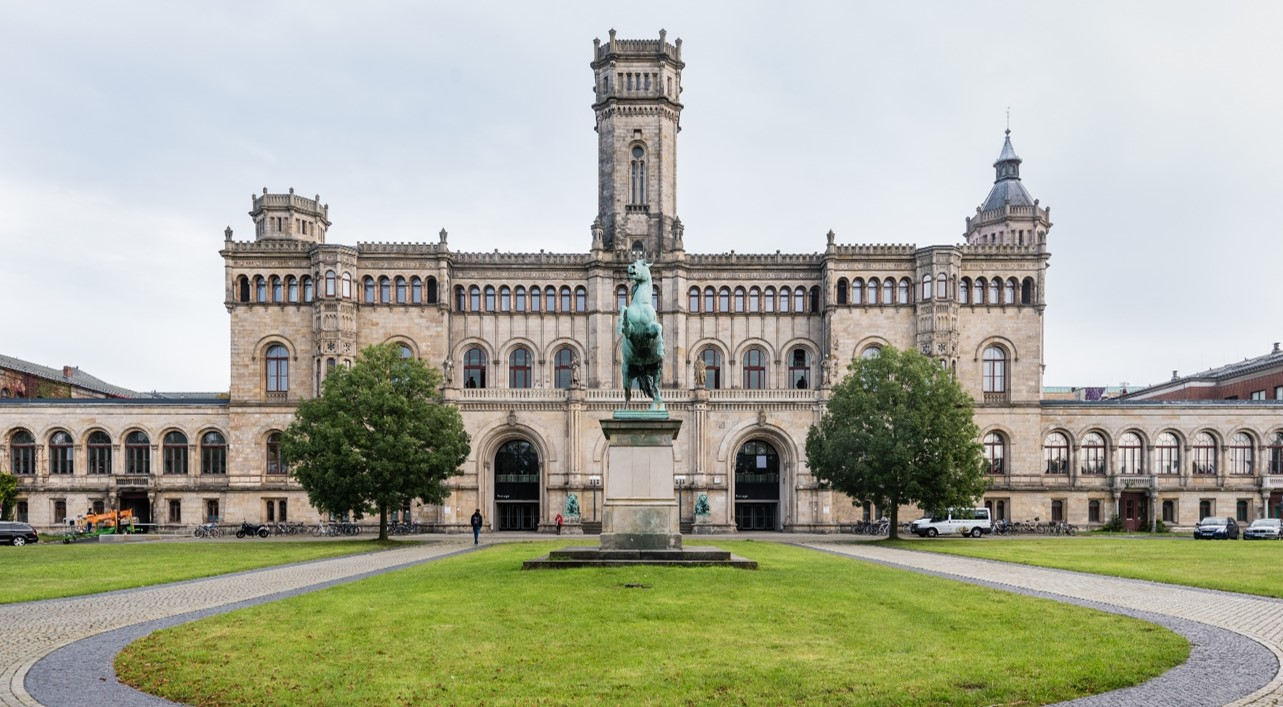
\includegraphics[width=0.65\textwidth]{figures/luh_default_presentation_title_image.jpg}}

% Title page: luhstyle
% \setbeamertemplate{title page}[luhstyle]
% % Add optional title image here
% \addtitlepageimage{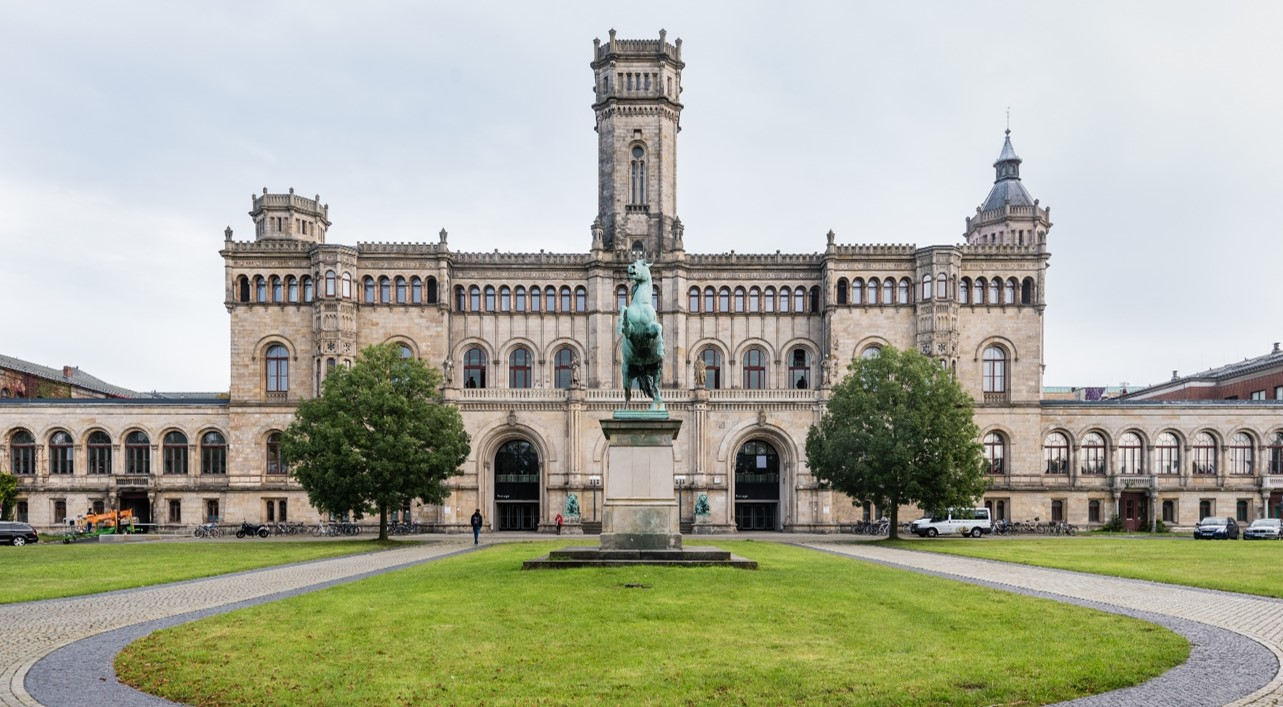
\includegraphics[width=0.75\textwidth]{figures/luh_default_presentation_title_image.jpg}}

\author[Abedjan \& Lindauer]{Ziawasch Abedjan \& Marius Lindauer\\[1em]
	
\includegraphics[height=\logoheight]{../latex_main/figures/luh_logo_rgb_0_80_155.pdf}\qquad
	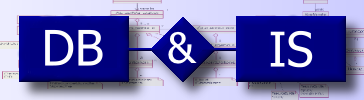
\includegraphics[height=\logoheight]{../latex_main/figures/DBIS_Kurzlogo.png}\qquad

\includegraphics[height=\logoheight]{../latex_main/figures/TNT_darkv4}\qquad

\includegraphics[height=\logoheight]{../latex_main/figures/L3S.jpg}	}
\date{Summer Term 2022; \hspace{0.5em} {
\includegraphics[height=1.5em]{../latex_main/figures/Cc-by-nc-sa_icon.svg.png}}; based on \href{https://ds100.org/fa21/}{[DS100]}
}


%%% Custom Packages
%----------------------------------------------------------------------
% Create dummy content
\usepackage{blindtext}

% Adds a frame with the current page layout. Just call \layout inside of a frame.
\usepackage{layout}


%%% Macros
%\renewcommand{\vec}[1]{\mathbf{#1}}
% \usepackage{bm}
%\let\vecb\bm

\title[Introduction]{DS: Data Sampling and Probability}
\subtitle{How to sample effectively, and how to quantify the samples we collect.}

\graphicspath{ {./figure/} }
%\institute{}


\begin{document}
	
	\maketitle
	
	\begin{frame}{Roadmap}
	    \begin{itemize}
	        \item Formalizing various ideas that pertain to sampling.
	        \begin{itemize}
	            \item Why we need to sample in the first place.
	            \item What it means for our sample to be biased.
	            \item How to prevent these biases in our samples.
	            \item What exactly a sampling frame is, and why choosing a good one is important.
	        \end{itemize}
	        \item Learning how to compute probabilities from samples.
	        \begin{itemize}
	            \item This will be continued into Lecture 3.
	        \end{itemize}
	    \end{itemize}
	\end{frame}
	
	\begin{frame}[c]{Data Science Lifecycle}
	    \begin{columns}
	        \begin{column}{.4\textwidth}
	        \begin{figure}
	            %\centering
	            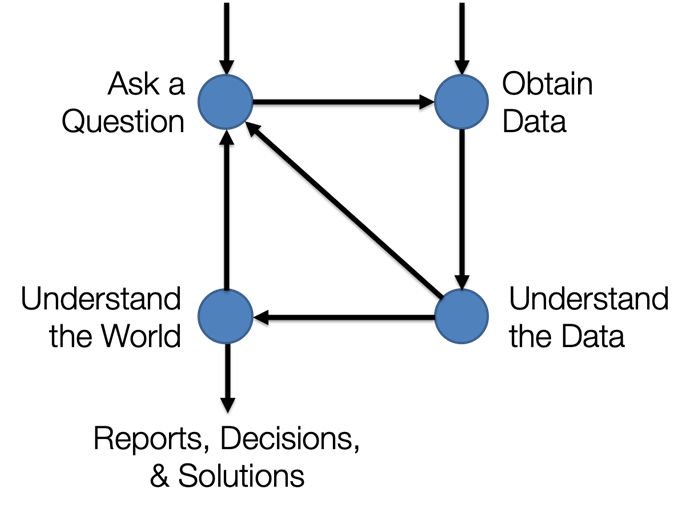
\includegraphics[scale=.6]{Bild1}
	        \end{figure}
	        \end{column}
	            
	        \begin{column}{.4\textwidth}
	        \bigskip
	        \bigskip
	        \bigskip
	        \bigskip
	            \centering
	            \begin{align*}
	                \text{We call this the} \\
	                \textbf{Data Science Lifecycle}
	            \end{align*}
	            
	        \end{column}

	    \end{columns}
	\end{frame}
	
	\begin{frame}{Question}
	    \begin{columns}
	        \begin{column}{.4\textwidth}
	        \bigskip
	        \bigskip
	        \bigskip
	        \bigskip
	         \centering
	            \begin{align*}
	                \text{Question: How many squirrels are there} \\
	                \text{in Central Park, New York City?}
	            \end{align*}
	       
	        \end{column}
	            
	        \begin{column}{.4\textwidth}
	            
	        \begin{figure}
	            %\centering
	            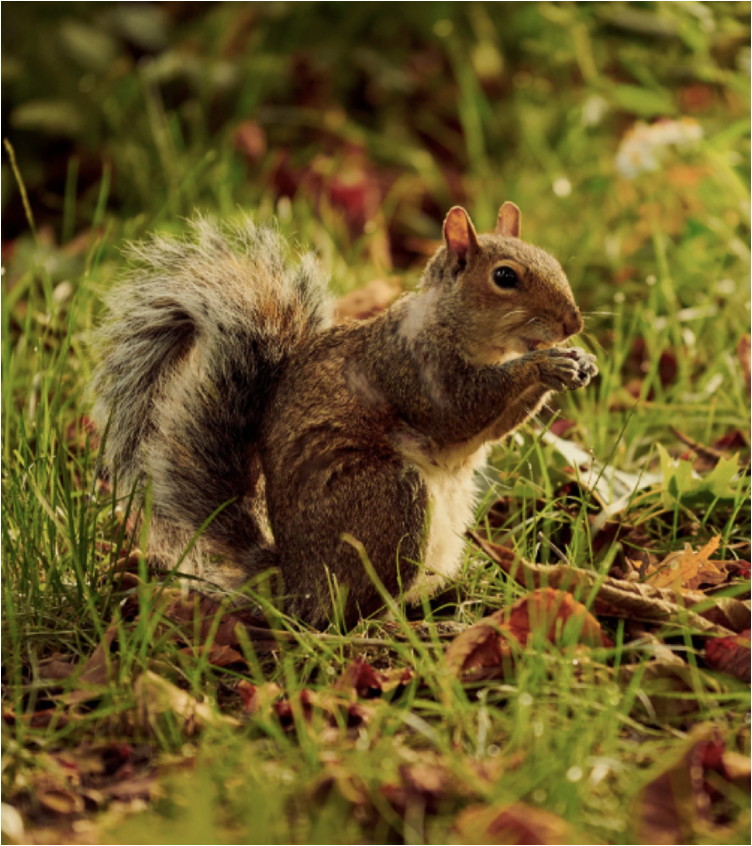
\includegraphics[scale=.45]{Bild2}
	        \end{figure}
	            
	        \end{column}
	        
	        \end{columns}
	\end{frame}
	
	
	\begin{frame}
	    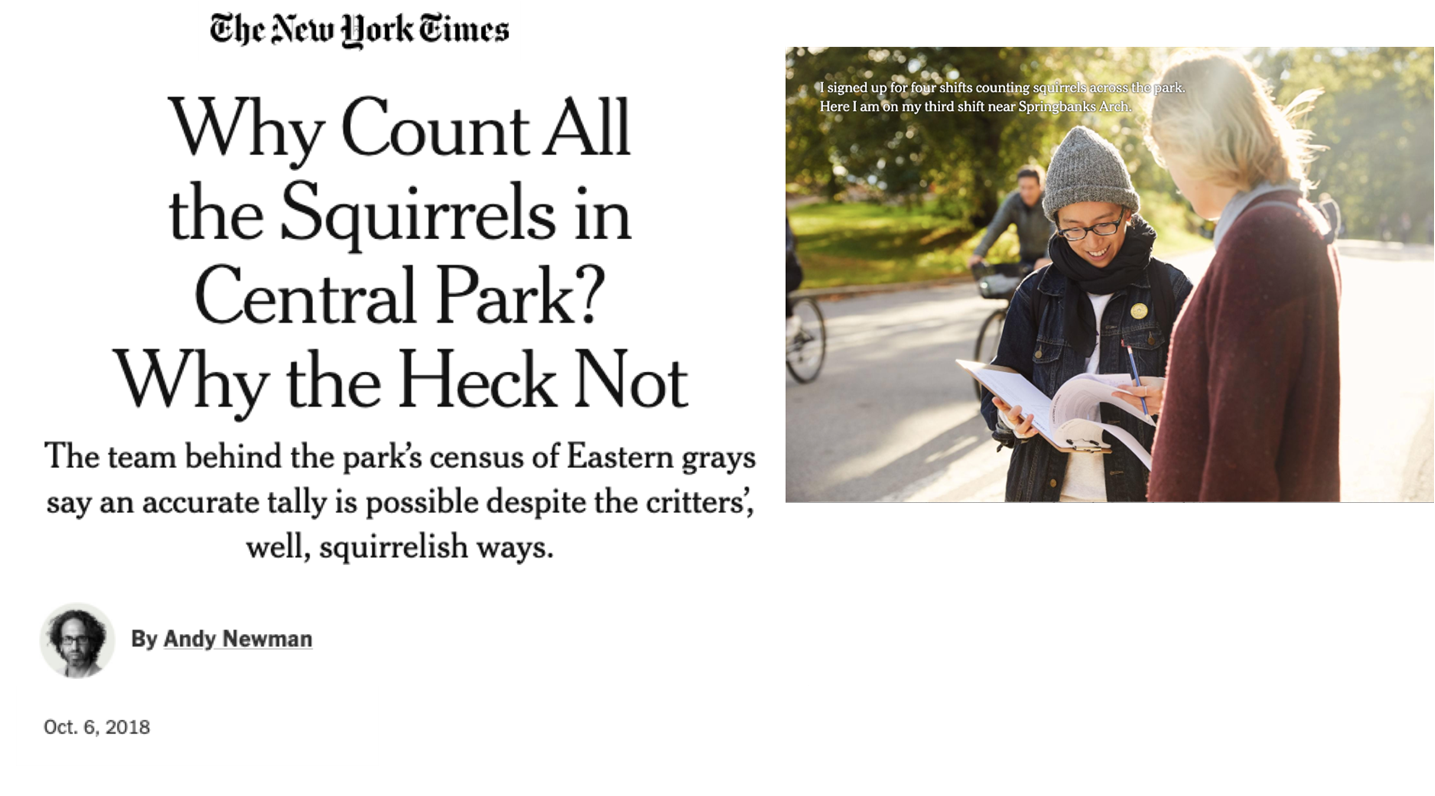
\includegraphics[scale=.6]{Bild3}
	\end{frame}
	
	\begin{frame}
	    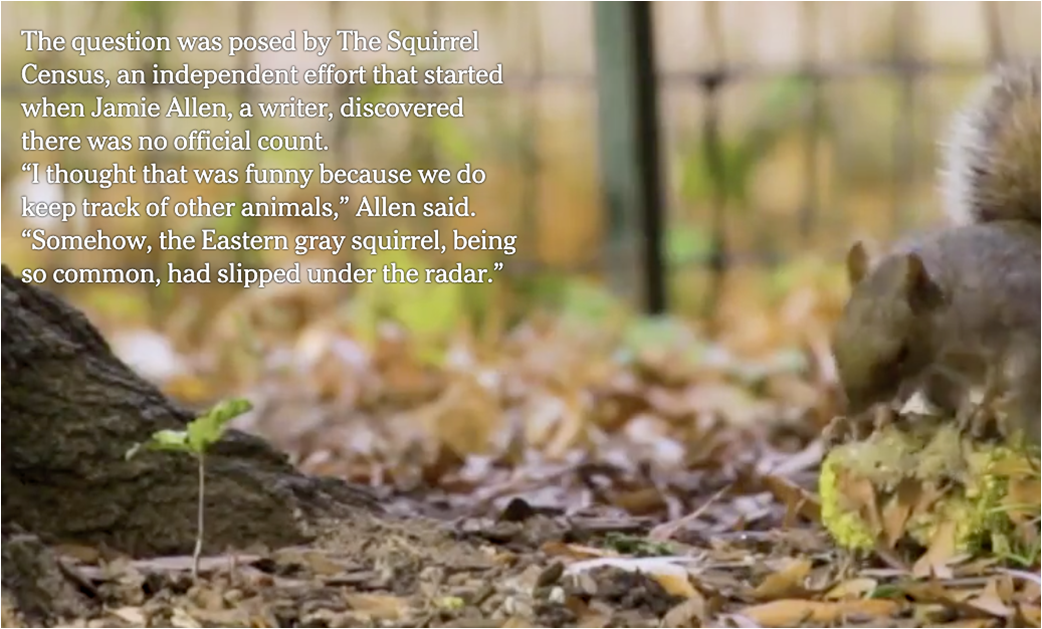
\includegraphics[scale=.6]{Bild4}
	\end{frame}
	
	
	\begin{frame}
	    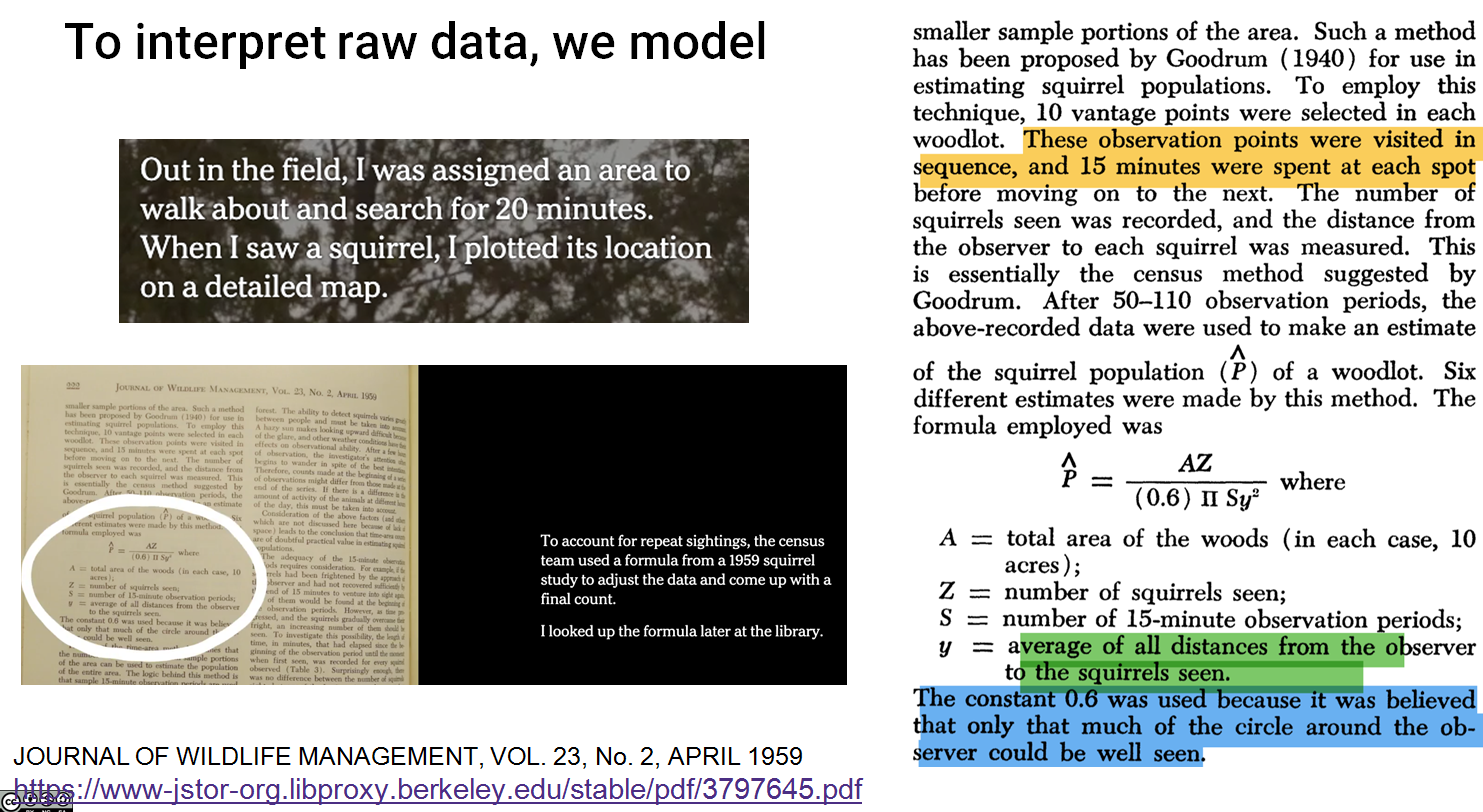
\includegraphics[scale=.37]{Bild5}
	\end{frame}
	
	
		\begin{frame}{The US Decennial Census}
	     \begin{columns}
	         \begin{column}{.4\textwidth}
	         \begin{itemize}
	             \item Was held in April 2020.
	             \item Counts every person living in all 50 states, DC, and US territories. (Not just citizens.)
	             \item Mandated by the Constitution. Participation is required by law.
	             \item Important uses:
	             \begin{itemize}
	                 \item Allocation of Federal funds.
	                 \item Congressional representation.
	                 \item Drawing congressional and state legislative districts.
	             \end{itemize}
	         \end{itemize}
	         

	         \end{column}
	         \begin{column}{.4\textwidth}
	                \begin{figure}
	                    \centering
	                    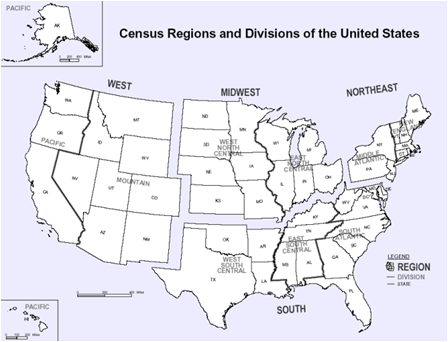
\includegraphics[scale=.5]{Bild6}
	                    \caption{data.census.gov}
	                \end{figure}
	                

	         \end{column}
	         
	         
	         
	     \end{columns}
	     In general: a census is “an official count or survey of a population, typically recording various details of individuals.”
	\end{frame}
	
	\begin{frame}{Surveys}
	    \begin{columns}
	         \begin{column}{.4\textwidth}
	         \begin{itemize}
	             \item A survey is a set of questions.
	             \begin{itemize}
	                 \item For instance: workers survey individuals and households.
	             \end{itemize}
	             \item What is asked, and how it is asked, can affect:
	             \begin{itemize}
	                 \item How the respondent answers.
	                 \item Whether the respondent answers.
	             \end{itemize}
	         \end{itemize}
	         There are entire courses on surveying!
            \begin{itemize}
                \item See Stat 152 at Berkeley (Sampling Surveys).
            \end{itemize}

	         \end{column}
	         \begin{column}{.4\textwidth}
	                \begin{figure}
	                    \centering
	                    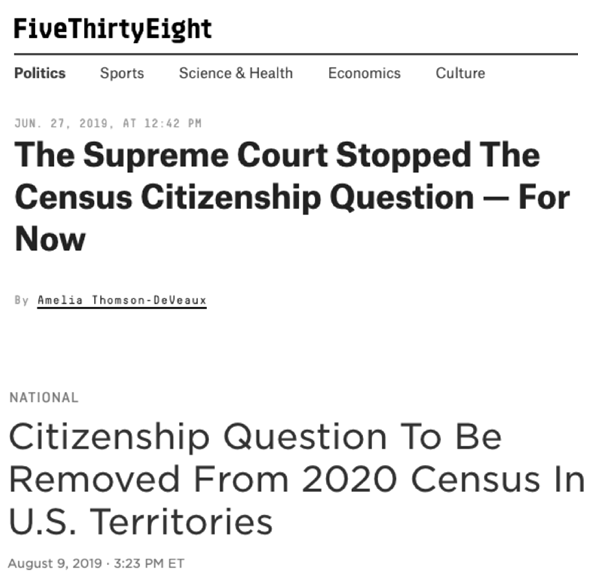
\includegraphics[scale=.35]{Bild7}
	                \end{figure}
	                

	         \end{column}
	     \end{columns}
	\end{frame}
	
	
	\begin{frame}{Issues with the US Decennial Census}
	    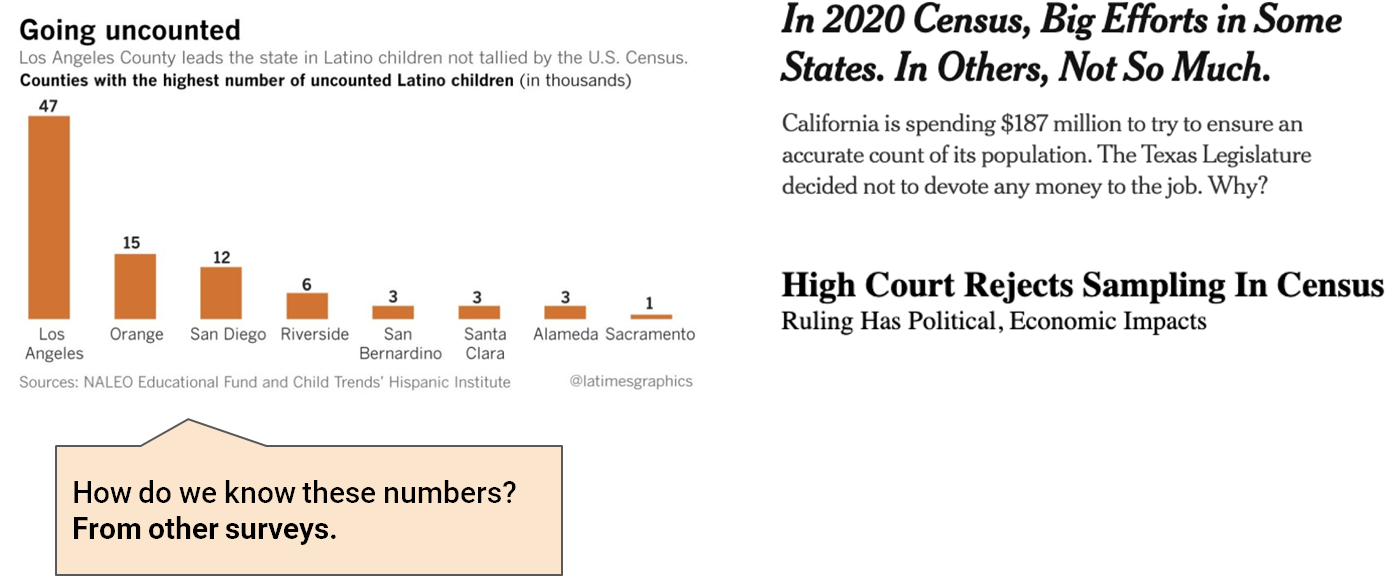
\includegraphics[scale=.4]{Bild8}
	\end{frame}
	
	
	
	
	\begin{frame}{Sampling from a finite population}
	    A census is great, but expensive and difficult to execute
	    \bigskip
	    A sample is a subset of the population.
        \begin{itemize}
            \item Samples are often used to make inferences about the population
            \item How you draw the sample will affect your accuracy.
            \item Two common sources of error:
            \begin{itemize}
                \item chance error: random samples can vary from what is expected, in any direction.
                \item bias: a systematic error in one direction.
            \end{itemize}
               \bigskip
               \bigskip
               We will now look at some types of non-random samples, before formalizing what it means for a sample to be random.

        \end{itemize}
	    
	\end{frame}
	
	\begin{frame}{Convenience samples}
	    \begin{columns}
	        \begin{column}{.4\textwidth}
	             A convenience sample is whoever you can get ahold of.
	             \begin{itemize}
	                 \item Not a good idea for inference!
	                 \item Haphazard ≠ random.
	                 \item Sources of bias can introduce themselves in ways you may not think of!
	             \end{itemize}
	                \bigskip
	                Convenience samples are not random.
	        \end{column}
	        \begin{column}{.4\textwidth}
	                Example: Suppose we have a cage of mice, and each week, we want to measure the weights of these mice. To do so, we take a convenience sample of these mice, and weigh them.
	                
	                \bigskip
	                Do you expect the weights of our sampled mice to be representative of all mice in our cage?
	                
	                \begin{figure}
	                    \centering
	                    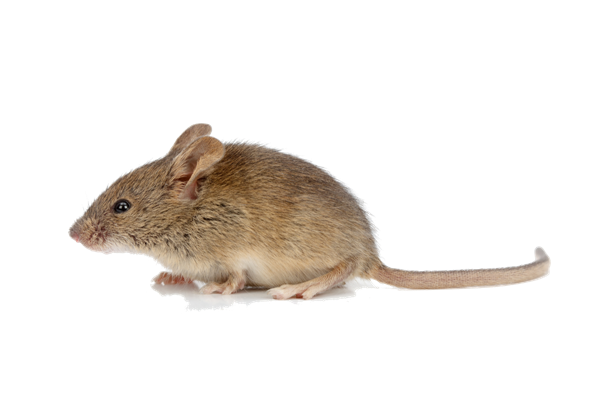
\includegraphics[scale=.4]{Bild9}
	                \end{figure}
	        \end{column}
	    \end{columns}
	\end{frame}
	
	\begin{frame}{Quota samples}
	    \begin{columns}
	        \begin{column}{.4\textwidth}
	            In a quota sample, you first specify your desired breakdown of various subgroups, and then reach those targets however you can.
	             \begin{itemize}
	                 \item For example: you may want to sample individuals in your town, and you may want the age distribution of your sample to match that of your town’s census results.
	             \end{itemize}
	                \bigskip
	               Quota samples are not random.

	        \end{column}
	        \begin{column}{.4\textwidth}
	               Issues with quota samples:
                   \begin{itemize}
                       \item Reaching quotas “however you can” is, as we saw in the previous slide, not random.
                       \item By setting quotas, you require that your sample look like your population with regards to just a few aspects – but not all!
                       \begin{itemize}
                           \item For example, if you set quotas for age, your sample might be representative of your population with regards to age.
                           \item What about gender? Ethnicity? Income?
                       \end{itemize}
 
                   \end{itemize}
	        \end{column}
	    \end{columns}
	\end{frame}

	\begin{frame}{Quality, not quantity!}
	     \begin{columns}
	        \begin{column}{.4\textwidth}
	            Try to ensure that the sample is representative of the population.
                   \begin{itemize}
                       \item Don’t just try to get a big sample.
                       \item If your method of sampling is bad, and your sample is big, you will have a big, bad sample!
                   \end{itemize}
                   \bigskip
                   This is a phenomenon you will explore in-depth in Homework 2, where you will perform an analysis of the 2016 US Presidential Elections.


	        \end{column}
	        \begin{column}{.4\textwidth}
	               \begin{figure}
	                   \centering
	                   
\includegraphics[scale=.4]{Bild10}
	                   \caption{Big bad Wolf}
	               \end{figure}
	        \end{column}
	        
	    \end{columns}
	\end{frame}
	
	
	
	\begin{frame}{Case study – 1936 Presidential Election}
	  \begin{figure}
	      \centering
	      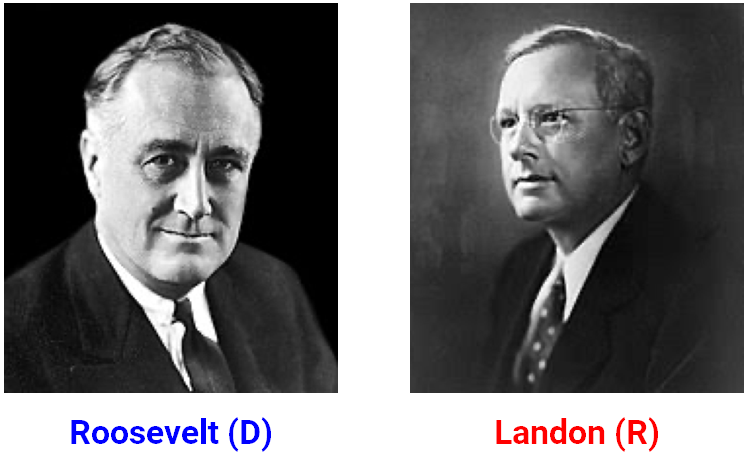
\includegraphics[scale=.4]{Bild11}
	  \end{figure}
	  In 1936, President Franklin D. Roosevelt (left) went up for re-election against Alf Landon (right). As is usual, polls were conducted in the months leading up to the election to try and predict the outcome.

	\end{frame}
	
	\begin{frame}{The Literary Digest}
	    \begin{columns}
	        \begin{column}{.4\textwidth}
	            The Literary Digest was a magazine. They had successfully predicted the outcome of 5 general elections coming into 1936.
	            \bigskip
	            
	            They sent out their survey to 10,000,000 individuals, who they found from:
	            \begin{itemize}
	                \item Phone books.
	                \item Lists of magazine subscribers.
	                \item Lists of country club members.
	            \end{itemize}
	        \end{column}
	        
	        \begin{column}{.5\textwidth}
	            \begin{figure}
	                \centering
	                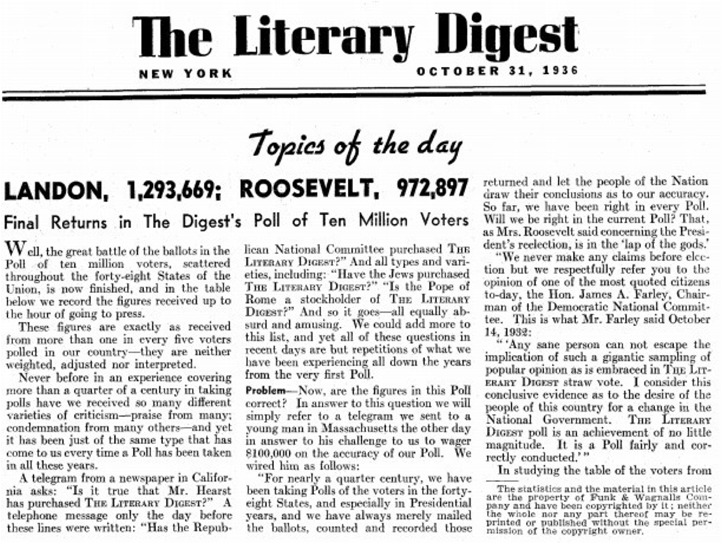
\includegraphics[scale=.58]{Bild12}
	            \end{figure}
	        \end{column}
	        
	    \end{columns}
	    
	\end{frame}
	
	
	\begin{frame}{The Literary Digest}
	    \begin{columns}
	        \begin{column}{.4\textwidth}
	            \bigskip


	            The Literary Digest’s prediction:
                \begin{align*}
                    \text{43\% Roosevelt, 57\% Landon}
                \end{align*}
                The actual outcome of the election:
                \begin{align*}
                    \text{61\% Roosevelt, 37\% Landon}
                \end{align*}
                How could this have happened? They surveyed 10 million people!
	        \end{column}
	        
	        \begin{column}{.5\textwidth}
	            \begin{itemize}
	                \item Their sample was not representative of the population.
	                \begin{itemize}
	                    \item They sampled people who owned phones, subscribed to magazines, and went to country clubs, who at the time were more affluent.
	                    \item These people tended to vote Republican (Alf Landon).
	                \end{itemize}
	                \item Only 2.4 million people actually filled out the survey!
	                \begin{itemize}
	                    \item 24\% response rate (low).
	                    \item Who knows how the other 76\% would have polled?
	                \end{itemize}
	            \end{itemize}
	        \end{column}
	        
	    \end{columns}
	    
	\end{frame}
	
	\begin{frame}{Gallup’s Poll}
	    \begin{columns}
	        \begin{column}{.4\textwidth}
	            George Gallup, a rising statistician, also made predictions about the impending 1936 elections. He predicted that Roosevelt would win with 56\% of the vote.
                \bigskip
                Not only was his estimate much closer than The Literary Digest’s estimate, but he did it with a sample size of only 50,000!
	        \end{column}
	        
	        \begin{column}{.5\textwidth}
	            George Gallup also predicted what The Literary Digest was going to predict, within 1\%. How was he able to predict what they were going to predict, with such accuracy?
                
                \begin{itemize}
                    \item He predicted that they would survey people in the phone book, people who subscribed to magazines, and who were part of country clubs.
                    \item So he sampled those same individuals!
                    \item He was able to predict their prediction by sampling only 3000 people.
                \end{itemize}
	        \end{column}
	        
	    \end{columns}
	    
	\end{frame}
	
	\begin{frame}{Summary of results}
	    \begin{columns}
	        \begin{column}{.6\textwidth}
	            \begin{tabular}{|l|l|l|}
	                \hline
	                 & \% Roosevelt & \#surveyed  \\
	               \hline
	               The Literary Digest poll  & 43\%  & 10,000,000\\
	               \hline
	               George Gallup’s poll & 56\% & 50,000\\
	               \hline
	               George Gallup’s\\ prediction of\\ Digest’s prediction & 44\% & 3,000\\
	               \hline
	               Actual election & 61\% & All voters\\
	               \hline
	            \end{tabular}
	        \end{column}
	        
	        \begin{column}{.4\textwidth}
	            Big samples aren’t always good!
                \begin{itemize}
                    \item What you need is a representative sample. 
                    \item If your sampling method is biased, those biases will be magnified with a larger sample size.
                \end{itemize}
	        \end{column}
	        
	    \end{columns}
	    
	\end{frame}
	
	
		\begin{frame}{Population, samples, and sampling frame}
	    \begin{columns}
	        \begin{column}{.4\textwidth}
	            \begin{itemize}
	                \item Population: The group that you want to learn something about.
                    \item Sampling Frame: The list from which the sample is drawn.
                    \begin{itemize}
                        \item If you’re sampling people, the sampling frame is the set of all people that could possibly end up in your sample.
                    \end{itemize}
                    \item Sample: Who you actually end up sampling. 
                    \begin{itemize}
                        \item A subset of your sampling frame.
                    \end{itemize}
	            \end{itemize}
	        \end{column}
	        
	        \begin{column}{.4\textwidth}
                \begin{figure}
                    \centering
                    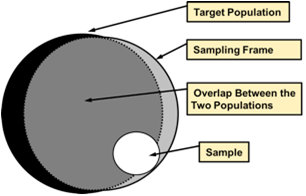
\includegraphics[scale=.5]{Bild13}\\
                    Note: There may be individuals in your sampling frame (and hence, your sample) that are not in your population!

                \end{figure}
	        \end{column}
	        
	    \end{columns}
	    
	\end{frame}
	
	
	\begin{frame}{Common Biases}
	    Selection Bias
        \begin{itemize}
            \item Systematically excluding (or favoring) particular groups.
            \item How to avoid: Examine the sampling frame and the method of sampling.
        \end{itemize}
        Response Bias
        \begin{itemize}
            \item People don’t always respond truthfully.
            \item How to avoid: Examine the nature of questions and the method of surveying.
        \end{itemize}
        Non-response Bias
        \begin{itemize}
            \item People don’t always respond.
            \item How to avoid: Keep your surveys short, and be persistent.
            \item People who don’t respond aren’t like the people who do!
        \end{itemize}
	\end{frame}
	
	
		\begin{frame}{Probability sampling}
	    \begin{columns}
	        \begin{column}{.4\textwidth}
	            Why? One reason is to reduce bias, but that’s not the main reason!
	            \begin{itemize}
	                \item Random samples can produce biased estimates of population characteristics.
	                \begin{itemize}
	                    \item For example, if we’re estimating the maximum of a population.
	                \end{itemize}
	                \item But with random samples we are able to estimate the bias and chance error.
	                \begin{itemize}
	                    \item We can quantify the uncertainty.
	                \end{itemize}
	            \end{itemize}
	        \end{column}
	        
	        \begin{column}{.5\textwidth}
	            For our purposes, probability samples and random samples will mean the same thing.
	            \bigskip
	            A probability sample is a type of sampling technique.
	        \end{column}
	        
	    \end{columns}
	    
	\end{frame}
	
	
		\begin{frame}{Probability sampling}
	    \begin{columns}
	        \begin{column}{.4\textwidth}
	            In order for a sample to be a probability sample:
	            \begin{itemize}
	                \item You must be able to provide the chance that any specified set of individuals will be in the sample.
	               \item All individuals in the population do not need to have the same chance of being selected.
	                \item You will still be able to measure the errors, because you know all the probabilities.
	            \end{itemize}
	        \end{column}
	        
	        \begin{column}{.5\textwidth}
	            Not all probability samples are necessarily good.
	            \bigskip
	            For instance, suppose I have three students: Allen, Kunal, Ishaan, and I want to sample two of them.
	            \begin{itemize}
	                \item I choose Allen with probability 1.
	                \item I choose either Kunal or Ishaan, each with probability $\frac{1}{2}$.
	            \end{itemize}
	            This is a probability sample (but it’s not great).

	        \end{column}
	        
	    \end{columns}
	    
	\end{frame}
	
	
		\begin{frame}{Some random sampling schemes}
	    \begin{columns}
	        \begin{column}{.7\textwidth}
	            A random sample with replacement is a sample drawn uniformly at random with replacement.

	            \begin{itemize}
	                \item Random doesn’t always mean “uniformly at random,” but in this specific context, it does.
	            \end{itemize}
	            A simple random sample is a sample drawn uniformly at random without replacement.
                 \begin{itemize}
	                \item Every individual has the same chance of being selected.
	                \item Every pair has the same chance as every other pair.
	                \item Every triple has the same chance as every other triple.
	                \item And so on.

	            \end{itemize}
	        \end{column}
	        
	        \begin{column}{.3\textwidth}
	            \begin{figure}
	                \centering
	                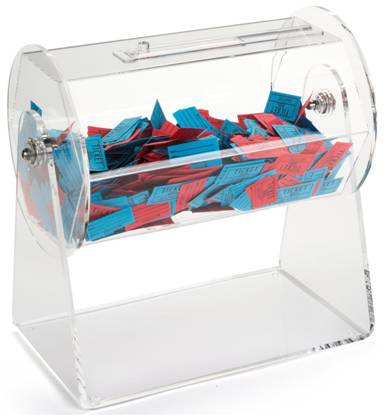
\includegraphics[scale=.5]{Bild14}
	            \end{figure}

	        \end{column}
	        
	    \end{columns}
	    
	\end{frame}
	
	
	
		\begin{frame}{Example scenario}
	    \begin{columns}
	        \begin{column}{.3\textwidth}
	            Consider the following sampling scheme:

	            \begin{itemize}
	                \item Suppose a class roster has 1200 students listed alphabetically.
	                \item Pick one of the first 10 students on the list at random.
	                \item To create your sample, take that student and every 10th student listed after that (e.g. Students 8, 18, 28, etc).
	            \end{itemize}
	            Pause here and answer these questions!
                 
	        \end{column}
	        
	        \begin{column}{.6\textwidth}
	           Is this a probability sample?\\
	           \bigskip
	           Does each student have the same probability of being selected?\\
	           \bigskip
	           Is this a simple random sample?


	        \end{column}
	        
	    \end{columns}
	    
	\end{frame}
	
		\begin{frame}{Example scenario}
	    \begin{columns}
	        \begin{column}{.3\textwidth}
	            Consider the following sampling scheme:

	            \begin{itemize}
	                \item Suppose a class roster has 1200 students listed alphabetically.
	                \item Pick one of the first 10 students on the list at random.
	                \item To create your sample, take that student and every 10th student listed after that (e.g. Students 8, 18, 28, etc).
	            \end{itemize}
                 
	        \end{column}
	        
	        \begin{column}{.6\textwidth}
	           Is this a probability sample?
	           \begin{itemize}
	               \item Yes. If my sample is [n, n + 10, n + 20, …, n + 1190], where 0 \leq n \leq 10, the probability of that sample is $\frac{1}{10}$
	               \item Otherwise, the probability is 0.
	               \item Only 10 possible samples!
	           \end{itemize}
	           Does each student have the same probability of being selected?\\
	           \bigskip
	           Is this a simple random sample?


	        \end{column}
	        
	    \end{columns}
	    
	\end{frame}
	
	\begin{frame}{Example scenario}
	    \begin{columns}
	        \begin{column}{.3\textwidth}
	            Consider the following sampling scheme:

	            \begin{itemize}
	                \item Suppose a class roster has 1200 students listed alphabetically.
	                \item Pick one of the first 10 students on the list at random.
	                \item To create your sample, take that student and every 10th student listed after that (e.g. Students 8, 18, 28, etc).
	            \end{itemize}

                 
	        \end{column}
	        
	        \begin{column}{.6\textwidth}
	           Is this a probability sample?
	           \begin{itemize}
	               \item Yes. If my sample is [n, n + 10, n + 20, …, n + 1190], where 0 \leq n \leq 10, the probability of that sample is $\frac{1}{10}$
	               \item Otherwise, the probability is 0.
	               \item Only 10 possible samples!
	           \end{itemize}
	           Does each student have the same probability of being selected?
	           \begin{itemize}
	               \item Yes. Each student is chosen with probability $\frac{1}{10}$. 
	           \end{itemize}
	           Is this a simple random sample?


	        \end{column}
	        
	    \end{columns}
	    
	\end{frame}
	
	\begin{frame}{Example scenario}
	    \begin{columns}
	        \begin{column}{.3\textwidth}
	            Consider the following sampling scheme:

	            \begin{itemize}
	                \item Suppose a class roster has 1200 students listed alphabetically.
	                \item Pick one of the first 10 students on the list at random.
	                \item To create your sample, take that student and every 10th student listed after that (e.g. Students 8, 18, 28, etc).
	            \end{itemize}
                 
	        \end{column}
	        
	        \begin{column}{.6\textwidth}
	           Is this a probability sample?
	           \begin{itemize}
	               \item Yes. If my sample is [n, n + 10, n + 20, …, n + 1190], where 0 \leq n \leq 10, the probability of that sample is $\frac{1}{10}$
	               \item Otherwise, the probability is 0.
	               \item Only 10 possible samples!
	           \end{itemize}
	           Does each student have the same probability of being selected?
	           \begin{itemize}
	               \item Yes. Each student is chosen with probability $\frac{1}{10}$. 
	           \end{itemize}
	           Is this a simple random sample?
                \begin{itemize}
                    \item No. The chance of selecting (8, 18) is 1/10; the chance of selecting (8, 9) is 0.
                \end{itemize}

	        \end{column}
	        
	    \end{columns}
	    
	\end{frame}
	
	
	\begin{frame}{A very common approximation}
	    \begin{itemize}
	        \item A common situation in data science:
	        \begin{itemize}
	            \item We have an enormous population.
	            \item We can only afford to sample a relatively small number of individuals.
	        \end{itemize}
	        \item If the population is huge compared to the sample, then random sampling with and without replacement are pretty much the same.
	        \begin{itemize}
	            \item For instance, if our population size is in the thousands, and we’re sampling 100 people, removing those 100 doesn’t change the population very much.
	        \end{itemize}
	        \item Probabilities of sampling with replacement are much easier to compute!
	    \end{itemize}
	\end{frame}
	
	
	
		\begin{frame}{The scenario}
	Binomial and multinomial probabilities arise when we:
	\begin{itemize}
	    \item Sample at random, with replacement.
	    \item Sample a fixed number (n) times.
	    \item Sample from a categorical distribution.
	    \begin{itemize}
	        \item For example, a bag of marbles in which 60\% are blue and 40\% are not blue.
	        \item Or where 60\% are blue, 30\% are green, and 10\% are red.
	    \end{itemize}
	    \item Want to count the number of each category that end up in our sample.
	\end{itemize}
	    Note: In this section, we will make use of the binomial coefficient and factorials. If you want a refresher on these, or want a more in-depth understanding, there’s an extra section at the end of this lecture that covers the derivation and some examples of it.

	\end{frame}
	
	
	\begin{frame}{Two categories}
	Suppose we sample at random with replacement 7 times from a bag of marbles, 60\% of which are blue and 40\% of which are not blue.

	\begin{itemize}
	    \item What is P(bnbbbnn)?
	    \begin{itemize}
	        \item By the product rule from Data 8, since the sample is drawn with replacement:
            \begin{align*}
                P(bnbbbnn) &= 0.6 \times 0.4 \times 0.6 \times 0.6 \times 0.6 \times 0.4 \times 0.4 \\
                &= (0.6)^4 (0.4)^3
            \end{align*}
	    \end{itemize}
	    \item How does P(4 blue, 3 not blue) compare to P(bnbbbnn)?
	    \begin{itemize}
	        \item P(4 blue, 3 not blue) > P(bnbbbnn).
	        \item Why? bnbbbnn is far more restrictive and specific than “4 blue, 3 not blue.”
	        \item There are several other ways to get “4 blue, 3 not blue” (for instance, bnnnbbb).
	    \end{itemize}
	\end{itemize}

	\end{frame}
	
	
		\begin{frame}{Binomial probabilities...}
	“4 blue, 3 not blue” can occur in several equally likely ways.\\                     For instance, P(bnbbbnn) = P(bnbbbnn) = P(bnbbbnn) = ... = (0.6)^4 (0.4)^3. \\         \bigskip
	    
	    P(4 blue, 3 not blue) is the total chance of all of those ways. The number of ways in which we can draw 4 blue marbles and 3 not blue marbles is

        \begin{align*}
            \binom{7}{4} = \frac{7!}{4!3!}
        \end{align*}
    and thus,
    \begin{align*}
        \text{P(4 blue, 3 not blue)} = \binom{7}{4}(0.6)^4 (0.4)^3 = \frac{7!}{4!3!}(0.6)^4 (0.4)^3
    \end{align*}

	\end{frame}
	
	
	\begin{frame}{Next time: random variables}
    	\begin{itemize}
    	    \item In the next lecture, we will formalize the notion of a random variable. Random variables arise naturally from this notion of a sample.
    	    \item We will then explore properties of random variables. 
    	    \begin{itemize}
    	        \item Expectation and variance.
    	        \item Various distributions.
    	        \item Sample means and sums.
    	    \end{itemize}
    	    \item We will then take a break from this discussion on sampling and probability, and switch gears to some of the more tools-focused ideas in this class. 
    	    \begin{itemize}
    	        \item SQL, pandas, regex, visualization, etc.
    	    \end{itemize}
    	    \item But not to worry – sampling, probability, and random variables in particular will reappear later in the semester.
    	\end{itemize}

	\end{frame}
	
	
	\begin{frame}{Disclaimer}
	    \begin{itemize}
	        \item This is not a class on probability or combinatorics. 
	        \begin{itemize}
	            \item In other words, this is not Stat 140 or CS 70.
	        \end{itemize}
	        \item This content on its own is not in scope.
	        \begin{itemize}
	            \item In other words, you will never be asked questions like “how many permutations of MISSISSIPPI are there”.
	            \item Instead, we present it in order to (re)explain where the binomial coefficient comes from.
	        \end{itemize}
	        \item This is purely meant to serve as a refresher, and is for your understanding only
	        \item Also, the video will walk through this material in perhaps a more natural fashion.
	    \end{itemize}
	\end{frame}
	
	\begin{frame}{Permutations}
	    Suppose I have five people, boringly named A, B, C, D, and E. In how many ways can I arrange them in a line?
	    \begin{itemize}
	        \item There are 5 options for who can end up first in line (anyone could).
	        \item Given that, there are 4 options for who can end up second in line.
	        \begin{itemize}
	            \item Could be anyone, other than whoever was first (5 - 1 = 4).
	        \end{itemize}
	        \item Given that, there are 3 options for who can end up third in line, and so on.
	    \end{itemize}
	    	       
	       Think of each blank as a position in line, and the number in the blank as the number of people that could end up there.\\
	       
	       \_\_5\_\_ \hspace{2cm}		\_\_4\_\_ \hspace{2cm}		\_\_3\_\_ \hspace{2cm}		\_\_2\_\_	 \hspace{2cm}	\_\_1\_\_

        The result is 5 * 4 * 3 * 2 * 1 = 120, which we denote as 5! (read “five factorial”). In general,\\
        \hspace{4cm} n! = n * (n - 1) * (n - 2) * … * 3 * 2 * 1


	\end{frame}
	
	\begin{frame}{Permutations}
	    How many ways can I arrange 3 of {A, B, C, D, E} in a line?

	    \begin{itemize}
	        \item 5 options for who is first.
	        \item 4 options for who is second.
	        \item 3 options for who is third.
	        \item Nobody after these three.
	    \end{itemize}

	      \hspace{4cm} \_\_5\_\_ \hspace{2cm}		\_\_4\_\_ \hspace{2cm}		\_\_3\_\_ 

       This result is 5 * 4 * 3 = 60. Note, we can also write 5 * 4 * 3 as\\
        \begin{align*}
            5 * 4 * 3 &= (5 * 4 * 3 * 2 * 1) / (2 * 1) \\
            &= 5! / 2! = 5! / (5 - 3)!
        \end{align*}
    What are the implications of this?
	\end{frame}
	
	
	\begin{frame}{Permutations}
	    In general: if I have n objects, and want to select k of them in a way that order matters, then the number of ways I can do this is

	    \begin{equation*}
	        \frac{n!}{(n-k)!}
	    \end{equation*}
        Again: this is not a class that covers counting!
        \begin{itemize}
            \item This result, by itself, will (almost certainly) never appear again in this class
            \item It’s more here to serve as an intermediate step in what comes next.
        \end{itemize}

	\end{frame}
	
		\begin{frame}{Combinations}
	    Now, suppose I want to select three people from {A, B, C, D, E}, but in a way that order does not matter.

        \begin{itemize}
            \item If order mattered, ABE, EAB, BAE, etc. would count as different arrangements.
            \item But if order does not matter, then the above three arrangements are all the same – they contain the same 3 people!
            \item If order does not matter, there are fewer ways to make our selections. 
        \end{itemize}
        How can we use our previous answer to help us here?
        \begin{itemize}
            \item How many times did we overcount?
            \item Each unique group of three people is counted 3! = 6 times.
            \begin{itemize}
                \item ABE, AEB, BAE, BEA, EAB, EBA are really all the same now.
                \item We need to divide our previous answer by the number of times we overcounted!
            \end{itemize}
        \end{itemize}

	\end{frame}
	
	
	\begin{frame}{Combinations}
	    Dividing our previous answer by 3! yields


        \begin{equation*}
            \frac{\frac{5!}{2!}}{3!} = \frac{5!}{2!3!}
        \end{equation*}
        This quantity is the number of ways we can select 3 objects from a set of 5, in a way that order does not matter.\\
        
        More generally, the number of ways we can select k objects from a set of n, in a way that order does not matter (and where k, n are both non-negative integers, and k \leq n) is:

        \begin{equation*}
            \binom{n}{k}= \frac{n!}{(n-k)!k!}
        \end{equation*}
        The symbol on the left is referred to as the binomial coefficient, and is read “n choose k.”

	\end{frame}
	
	
	\begin{frame}{Combinations}
	    Here are some examples on how we can (and will) use the binomial coefficient.
        \begin{itemize}
            \item How many ways can we flip a coin (whose flips are independent of one another) 4 times and see 2 heads?
            \begin{itemize}
                \item Equivalent question: how many different ways can we order the string “HHTT”?
                \item There are 4 “positions.” Choose 2 of them to be H (the remaining 4 will be T).
                \item This is 4 choose 2, or 6. (Enumerated: HHTT, HTHT, HTTH, TTHH, THTH, THHT.)
            \end{itemize}
            \item Suppose we have a bag of marbles that contains marbles, some of which are blue. How many ways can we draw 7 marbles, such that 4 are blue and 3 are not blue?
            \begin{itemize}
                \item We have 7 draws. Choose 4 of them to be blue (the remaining automatically are not).
                \item This is 7 choose 3, or 35 
            \end{itemize}
            \item Note: The above answers (and algebra) imply that $\binom{n}{k}=\binom{n}{n-k}$
            \begin{itemize}
                \item Choosing k successes is equivalent to choosing n - k failures.
            \end{itemize}
        \end{itemize}

	\end{frame}
	
	\begin{frame}{What about order?}
	    \begin{columns}
	        \begin{column}{.4\textwidth}
	            You may be wondering – why did we use the binomial coefficient to determine the number of orderings of 2 heads and 2 tails (HHTT, HTHT, HTTH, TTHH, THTH, THHT), when the whole point was that order doesn’t matter?\\
	            \bigskip
	            The order in which we declare the positions is what doesn’t matter here. The contents of each position, though, do matter. 
	        \end{column}
	        
	        \begin{column}{.5\textwidth}
	           \begin{figure}
	               \centering
	               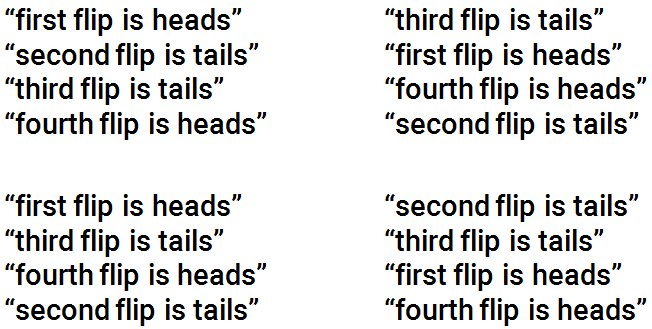
\includegraphics[scale=.3]{Bild15}
	           \end{figure}
	           These are all equivalent! They all equate to the ordering HTTH.\\
	           
	           The order in which you tell me what flip goes where is not of importance. This is why we use choosing here.

	        \end{column}
	        
	    \end{columns}
	    
	\end{frame}
	
	\begin{frame}{Another interpretation}
	    How many ways can we flip a coin (whose flips are independent of one another) 4 times and see 2 heads?
        \begin{itemize}
            \item Equivalent problem to determining the number of rearrangements of HHTT.
            \item Let’s label them uniquely: H1, H2, T1, T2.
            \item There are 4 objects, so there are 4! orders.
            \item But, some of these orderings are really the same!
            \begin{itemize}
                \item “H1 H2 T1 T2” is really the same as “H2 H1 T2 T1” and “H1 H2 T2 T1.”
                \item These should all count as one “ordering.”
                \item There are 2! ways to arrange the two Hs amongst themselves.
                \item There are 2! ways to arrange the two Ts amongst themselves.
            \end{itemize}
            \item Dividing out the repetition yields, as we saw before, $\frac{4!}{2!2!}$
        \end{itemize}

	\end{frame}
	
	\begin{frame}{Extension to multiple categories}
	    How many ways can I select 7 marbles from a bag such that 4 are blue, 2 are green, and 1 is red? (e.g. bgbbbgr, bbbrgbg, brbgbgb, etc.)\\
	    \bigskip
	    Again, there are two interpretations.

        \begin{align*}
            \binom{7}{4}\cdot \binom{3}{2} \cdot \binom{1}{1} \qquad \qquad \frac{7!}{4!2!1!}
        \end{align*}

	\end{frame}
	
	
	\begin{frame}{Extension to multiple categories}
	    How many ways can I select 7 marbles from a bag such that 4 are blue, 2 are green, and 1 is red? (e.g. bgbbbgr, bbbrgbg, brbgbgb, etc.)\\
	    \bigskip
	    Again, there are two interpretations.

        \begin{align*}
            \binom{7}{4}\cdot \binom{3}{2} \cdot \binom{1}{1} \qquad \qquad \frac{7!}{4!2!1!}
        \end{align*}

	\end{frame}
	
	
	\begin{frame}{Extension to multiple categories}
	    How many ways can I select 7 marbles from a bag such that 4 are blue, 2 are green, and 1 is red? (e.g. bgbbbgr, bbbrgbg, brbgbgb, etc.)\\
	    \bigskip
	    Again, there are two interpretations.

        \begin{figure}
                \centering
                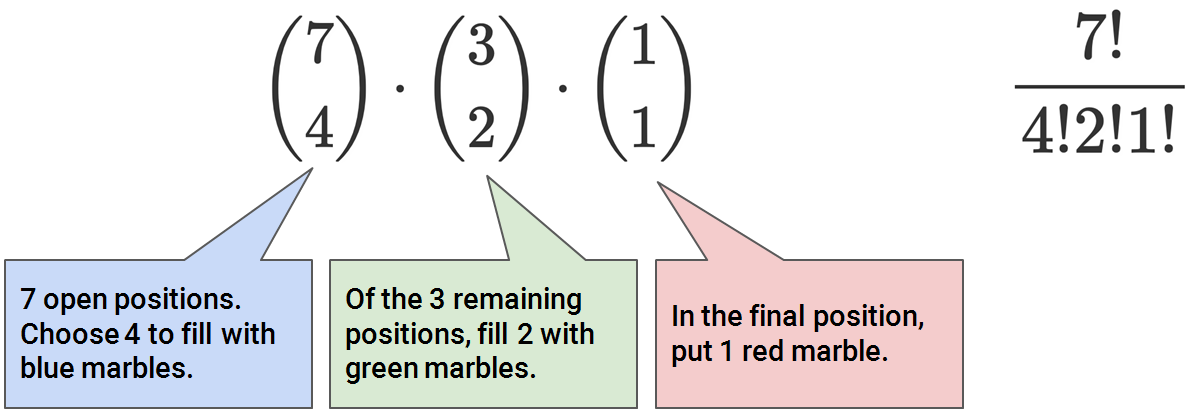
\includegraphics[scale=.4]{Bild16}
            \end{figure}


	\end{frame}
	
	
	
	
	\begin{frame}{Extension to multiple categories}
	    How many ways can I select 7 marbles from a bag such that 4 are blue, 2 are green, and 1 is red? (e.g. bgbbbgr, bbbrgbg, brbgbgb, etc.)\\
	    \bigskip
	    Again, there are two interpretations.
            \begin{figure}
                \centering
                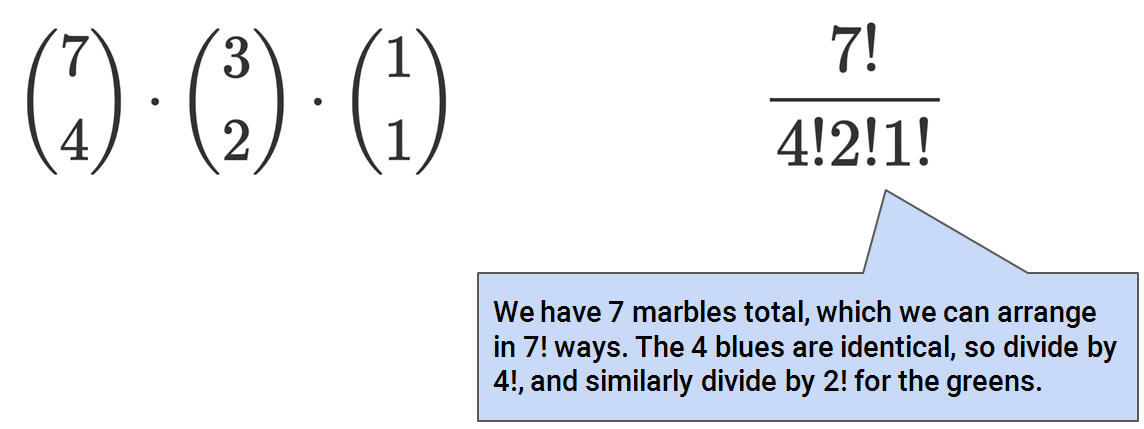
\includegraphics[scale=.4]{Bild17}
            \end{figure}

	\end{frame}
	
	
	
	
	
	\begin{frame}{Extension to multiple categories}
	    How many ways can I select 7 marbles from a bag such that 4 are blue, 2 are green, and 1 is red? (e.g. bgbbbgr, bbbrgbg, brbgbgb, etc.)\\
	    \bigskip
	    Again, there are two interpretations.

        \begin{align*}
            \binom{7}{4}\cdot \binom{3}{2} \cdot \binom{1}{1} \qquad  = \qquad \frac{7!}{4!2!1!}
        \end{align*}
        Unsurprisingly, they are equal!
	\end{frame}
\end{document}